\section{Supplement B parity examples}\label{app:application-si}

This companion records downstream verification and application rows from the cited native ledgers. Every row begins from the native side of the ledger; familiar labels, SI quantities, decimal compressions, or sector-comparative renderings are attached after the cited native row has been fixed.

\subsection{Familiar-label verification bindings}\label{app:familiar-bindings}
\paragraph{Application binding table.} Each row begins from the cited native row and then records the attached downstream report binding.

\begin{center}
\begin{tabularx}{\linewidth}{@{}lXXl@{}}
\toprule
Native structural key & Native rows to verify & Familiar verification label & Status \\
\midrule
\texttt{tetron:1:2:6} & $\lambda$-band, $B^*$, $R_{\mathrm{rest}}$, cadence & electron & verification binding \\
\texttt{tetron:1:2:8} & $\lambda$-band, $B^*$, $R_{\mathrm{rest}}$, cadence & muon & verification binding \\
\texttt{tetron:1:2:10} & $\lambda$-band, $B^*$, $R_{\mathrm{rest}}$, cadence & tau & verification binding \\
\texttt{tetron:3:3:6} & shell signature, $B^*$, confinement, $R_{\mathrm{rest}}$ & proton & verification binding \\
\texttt{tetrad:3:4:6} & shell signature, $B^*$, confinement, $R_{\mathrm{rest}}$ & neutron & verification binding \\
\texttt{duon}/\texttt{duad} & push/pull, export witness, cadence & radiation / exchange family & verification binding \\
\bottomrule
\end{tabularx}
\end{center}

\subsection{SI / decimal parity routing}\label{app:si-routing}
\paragraph{SI / decimal routing.} Any SI, decimal, or sector-comparative rendering is recorded here from a cited native row.

\begin{center}
\begin{tabularx}{\linewidth}{@{}lXl@{}}
\toprule
Native source row & Downstream rendering target & Notes \\
\midrule
E4 native rest-channel row & put-to-seconds, Hz, J, kg, MeV/$c^2$ dictionaries & downstream dictionary rendering \\
E5 $B^*$ ladder row & decimal ladder summaries / attractor plots & non-premise compression \\
E6 collision/export row & downstream sector/event illustrations & downstream application rendering \\
E7 field-property row & real-world comparison dashboards / parity tables & native row followed by application rendering \\
\bottomrule
\end{tabularx}
\end{center}

\subsection{Real-world application rows}\label{app:realworld-routing}
\paragraph{Application rows.} Real-world application rows begin from the native key, cited window, shell signature, $B^*$, cadence, torsional residual, and rest-channel data, and then record the attached application-side labels or unit conversions.

\begin{center}
\begin{tabularx}{\linewidth}{@{}lX@{}}
\toprule
Application class & Required native starting columns \\
\midrule
Familiar field/particle parity & key, cited window, $\lambda$-band, shell signature, $B^*$, $R_{\mathrm{rest}}$, $R^{(\mathrm{putz})}_{\mathrm{rest}}$, cadence, torsional residual \\
Laboratory / engineering parity & key, cited window, shell predicate, export witness, native rates, declared dictionary map id \\
Scale-comparative demonstrations & key, shell signature, cadence spectrum, confinement witness, support signature, native rates \\
\bottomrule
\end{tabularx}
\end{center}


\subsection{Feynman-style dictionary rendering}\label{app:feynman-dict}
\paragraph{Dictionary rendering.} The collision/export rows may also be rendered in a Feynman-style dictionary view after the cited native row has been fixed. The rendering below is a downstream compression of the same integer ledgers recorded for Example~E6 in the native supplement; it adds no premise to the native theorem space.

\begin{center}
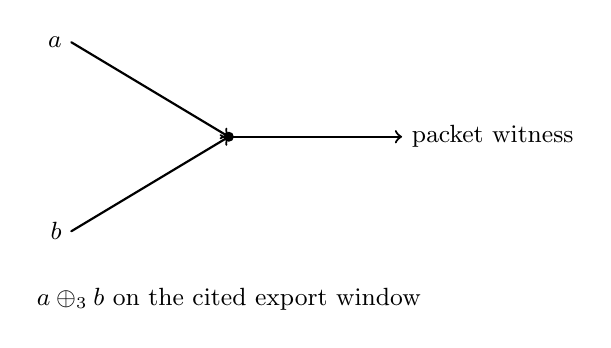
\begin{tikzpicture}[x=1cm,y=1cm, line cap=round, line join=round, every node/.style={font=\small}]
  % vertex
  \filldraw[black] (0,0) circle (1.6pt);
  % incoming/outgoing legs
  \draw[thick,->] (-2,1.2) -- (0,0);
  \draw[thick,->] (-2,-1.2) -- (0,0);
  \draw[thick,->] (0,0) -- (2.2,0);
  \node[left] at (-2,1.2) {$a$};
  \node[left] at (-2,-1.2) {$b$};
  \node[right] at (2.2,0) {packet witness};
  \node[below] at (0,-1.8) {$a\oplus_3 b$ on the cited export window};
\end{tikzpicture}
\end{center}

\paragraph{Native anchor.} Use this rendering only with an explicit citation to the corresponding native collision/export row and its cut residual check.


\subsection{Example E10: 3-node recurrent ring / recurrent-network rendering}\label{app:e10-neural}
\paragraph{Purpose.} Demonstrate that a small recurrent network is representable as a motif / closure + wavelet-propagation ledger in which projected non-Markov behavior is a representation adequacy issue and lag/backlog is a clock channel rather than kernel bias.
\paragraph{Depends on.} Native collision/export bookkeeping, backlog / forced-dwell bookkeeping, and the CK-mismatch witness on the cited projected stream.
\paragraph{Native row(s).}
{\footnotesize
\begin{center}
\begin{tabular}{@{}llllllll@{}}
\toprule
Row & topology & $u_{(\mathrm{loss})}$ [trit/put] & $B^*$ & $\widehat\Lambda$ & $R_{\mathrm{rest}}^{(\mathrm{putz})}$ & CK mismatch & $\mathcal R_{\mathrm{cut}}$ \\
\midrule
E10.N1 & 3-node ring & $0.4887777778$ & $2$ & $3$ & $0.0888534592$ & $0.0638525823$ & $0$ \\
\bottomrule
\end{tabular}
\end{center}}
\paragraph{Backlog / dwell slice.}
{\footnotesize
\begin{center}
\begin{tabular}{@{}lllllll@{}}
\toprule
$t$ & node & $\tau_\alpha$ & $\tau_\omega$ & delay [put] & hidden mode & backlog \\
\midrule
0 & A & $+1$ & $0$ & $3$ & $0$ & $1$ \\
1 & B & $+1$ & $0$ & $2$ & $0$ & $2$ \\
2 & -- & $0$ & $0$ & $0$ & $0$ & $2$ \\
3 & -- & $0$ & $-2$ & $0$ & $0$ & $0$ \\
4 & C & $-1$ & $0$ & $2$ & $0$ & $1$ \\
\bottomrule
\end{tabular}
\end{center}}
\paragraph{Dictionary rendering.} The same native row may be rendered as a three-node recurrent network with node activations and signed transport on the ring $A\to B\to C\to A$. This rendering is downstream and follows the cited native row.
\begin{center}
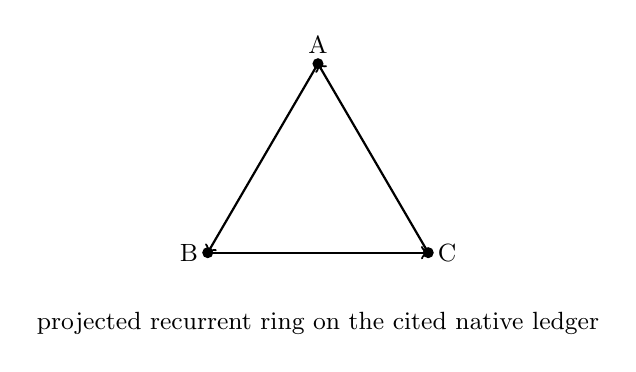
\begin{tikzpicture}[x=1cm,y=1cm, every node/.style={font=\small}]
  \coordinate (A) at (0,1.6);
  \coordinate (B) at (-1.4,-0.8);
  \coordinate (C) at (1.4,-0.8);
  \draw[thick,->] (A) -- (B);
  \draw[thick,->] (B) -- (C);
  \draw[thick,->] (C) -- (A);
  \fill (A) circle (2pt) node[above] {A};
  \fill (B) circle (2pt) node[left] {B};
  \fill (C) circle (2pt) node[right] {C};
  \node at (0,-1.7) {projected recurrent ring on the cited native ledger};
\end{tikzpicture}
\end{center}
\paragraph{Audit cues.} Use the CK residual $\|P^{(2)}-P^{(1)}P^{(1)}\|_F$, backlog/dwell columns, and cut residual to distinguish hidden-state projection effects from kernel bias.

\subsection{Example E11D: downstream decimal / optics-style rendering}\label{app:e11-dict}
\paragraph{Dictionary rendering.} After the cited native E11 row is fixed, one may record decimal or optics-style renderings of the same ratios. These renderings are downstream only.
{\footnotesize
\begin{center}
\begin{tabular}{@{}lllllllll@{}}
\toprule
row & $q_{\mathrm{eff}}$ & $\widehat q_{\mathrm{eff}}$ & $\eta_{\mathrm{out}}$ & $\eta_{\mathrm{mid}}$ & $\eta_{\mathrm{tot}}$ & $u_{(\mathrm{loss})}$ & $v$ & $n_{\mathrm{ref}}$ \\
\midrule
E11.q$-1$ & $-1$ & $-1.000000$ & $0.749647$ & $0.752841$ & $0.750282$ & $0.375061$ & $0.840820$ & $1.172967$ \\
E11.q$-1/2$ & $-1/2$ & $-0.493060$ & $0.481027$ & $0.625493$ & $0.547375$ & $0.354369$ & $0.695801$ & $1.329007$ \\
E11.q$0$ & $0$ & $0.026572$ & $0.267368$ & $0.518727$ & $0.441348$ & $0.369305$ & $0.539551$ & $1.546828$ \\
E11.q$1/2$ & $1/2$ & $0.511600$ & $0.524917$ & $0.621769$ & $0.568376$ & $0.367971$ & $0.698242$ & $1.335072$ \\
E11.q$1$ & $1$ & $1.000000$ & $0.750535$ & $0.742188$ & $0.748741$ & $0.368562$ & $0.828613$ & $1.175660$ \\
\bottomrule
\end{tabular}
\end{center}}
\paragraph{Native anchor.} These decimals are convenience renderings of the cited native E11 ledger and must not be used as operator premises.
